% Chapter Template

\chapter{CFD Analysis} % Main chapter title

\label{cfd} % Change X to a consecutive number; for referencing this chapter elsewhere, use \ref{ChapterX}

\lhead{\emph{CFD analysis}} % Change X to a consecutive number; this is for the header on each page - perhaps a shortened title

%----------------------------------------------------------------------------------------
%	SECTION
%----------------------------------------------------------------------------------------
\section{Case preprocessing} \label{casepre}

CFD analyses for generating raw pressure field data are performed in ANSYS Fluent 17.2 software on Prometheus HPC cluster located in Kraków. Access for this infrastructure was granted by PLGrid infrastructure. Calculations were run on 5 nodes of 24CPU cores and 128GB RAM each \citep{prometheus}, which resulted in decomposition to 120 cores, resulting in allocating around 110 thousand cells to a single HPC core.

Following, is the numerical setup applicable to all performed analyses. The setup corresponds to "peak efficiency conditions" given by the experimental study.

Material used in the analysis resembles standard air modeled as ideal gas as in equation with following properties described in table \ref{tab:stdair} 

\begin{table}[htb!]
\centering
\caption{Standard air properties} \label{tab:stdair}
\begin{tabular}{ r r l }
$C_p$ & 1006.43 & $\frac{J}{kg \cdot K}$ \\
$\lambda$ & 0.0242 & $\frac{W}{m \cdot K}$ \\
$\mu$ & 1.7894e-05 & $\frac{kg}{m \cdot s}$ \\
$M$ & 28.966 & $\frac{kg}{kmol}$ \\
\end{tabular}
\end{table}

\begin{equation} \label{eq:stadair}
p V = n R T
\end{equation}

Analysis operating pressure is set to 0 Pascal, which is a standard practice in compressible flow CFD.

Internal mesh zone is set as "frozen rotor" - stationary reference frame. Although no mesh motion is implied, the effect of Coriolis accelerations and centrifugal acceleration will be taken into account by adding respective acceleration components to momentum equations as described in chapter \ref{approach}. The rotational velocity is set to 1680 rad/s.

Following boundary conditions were applied to the mesh boundaries. Following setup is typical for compressible flow CFD.

\begin{table}[htb!]
\centering
\caption{Test case boundary conditions} \label{tab:testbcs}
\begin{tabular}{ | l | l | r l | } \hline
Boundary marker & Boundary type & & \\ \hline \hline
Inlet & Pressure Inlet & 101350  & Pa\\ \hline
Outlet & Pressure Outlet & 102000 & Pa \\ \hline
Hub & Movig wall & 1680 & rad/s \\ \hline
Blade & Moving wall & 1680 & rad/s \\ \hline
Casing & Stationary wall & &  \\ \hline
Internal profiles & Internal & & \\ \hline
Periodic boundaries & Interface & & \\ \hline 
\end{tabular}
\end{table}

Moving wall boundaries represent the rotational velocity of the compressor blade and are necessary for stationary reference frame formulation. Boundary condition setup is no different to usual setups of analyses of such kind.

\section{Flowfield initialization \& RANS}
RANS analysis is not suitable for generating acoustic nearfield data as the method averages the fluctuations over time (chapter \ref{approach}). Yet, the method generates an initial flowfield at a relatively low computational cost. Furthermore the RANS analysis will provide initial validation results for the test case and solver settings.

The solver is set up to steady-state, density based solver with $k-\omega SST$ turbulence model. Such setup is a go-to setup for nearly all compressible aerodynamics CFD done in the author's institute.

Flowfield is initialized at first with constant values populated from the "inlet" boundary condition patch. Next a Fast-Multi-Grid initialization is performed to generate coarsened flowield. The analysis is then processed by first, second and third order discretisation schemes for all of the conservation values, up to a given residual value. It must be noted, that for second and third order scheme analyses, convergence criteria may not be reached. Should this case occur, the analysis is stopped once the residual plots reach a plateau and the resulting flowfield is considered acceptable. Once the third order scheme analysis is completed, data is acquired from inlet and outlet boundary conditions, and the constant pitch vs. span streamlines.

%----------------------------------------------------------------------------------------
%	SECTION 2
%----------------------------------------------------------------------------------------

\section{DDES analysis}

Sed ullamcorper quam eu nisl interdum at interdum enim egestas. Aliquam placerat justo sed lectus lobortis ut porta nisl porttitor. Vestibulum mi dolor, lacinia molestie gravida at, tempus vitae ligula. Donec eget quam sapien, in viverra eros. Donec pellentesque justo a massa fringilla non vestibulum metus vestibulum. Vestibulum in orci quis felis tempor lacinia. Vivamus ornare ultrices facilisis. Ut hendrerit volutpat vulputate. Morbi condimentum venenatis augue, id porta ipsum vulputate in. Curabitur luctus tempus justo. Vestibulum risus lectus, adipiscing nec condimentum quis, condimentum nec nisl. Aliquam dictum sagittis velit sed iaculis. Morbi tristique augue sit amet nulla pulvinar id facilisis ligula mollis. Nam elit libero, tincidunt ut aliquam at, molestie in quam. Aenean rhoncus vehicula hendrerit.

%-----------------------------------
%	SECTION
%-----------------------------------
\section{Validation of the results}
Reference \citep{r67laser} provides a very extensive set of validation data for whole passage. The quoted study presents results of LDA measurements of the NASA R67 compressor for relative mach number and relative flow angle at constant pitch and constant chord lines intersecting with blade span lines at 10\% intervals. Constant pitch line is derived from the blade's suction surface: 0\% percent pitch is the suction surface of one blade, 100\% pitch is the suction surface of the adjacent blade. Constant chord lines are used to plot blade-to-blade distributions of given parameters at intersection of span and constant z-coordinate surface (\ref{fig_LA}).

\begin{figure}[h!]
\centering % bo \centering nie wstawia dodatkowego odstępu
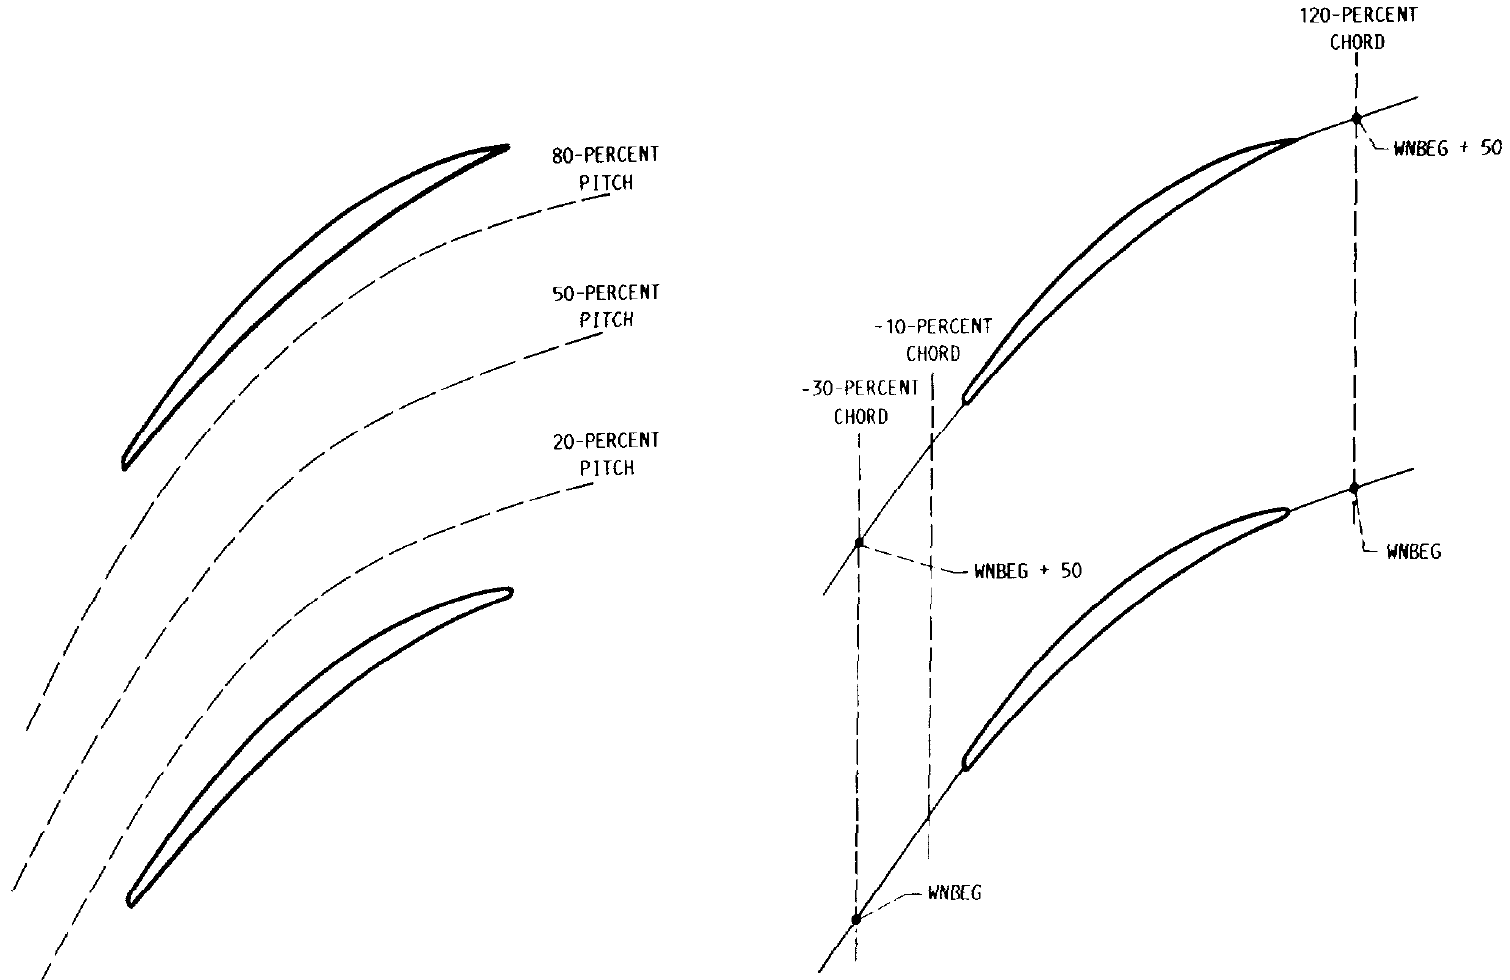
\includegraphics[width=0.85\textwidth]{Pictures/LA.png}
\caption{Schematic representation of constant pitch (left) and constant chord (right) to plot data \citep{r67laser}}
\label{fig_LA}
\end{figure}

This approach produces a very large number of plots, that are unnecessary for this particular thesis. To validate the presented RANS analysis, the constant pitch surfaces for 20\%, 50\% and 80\% pitch are combined with 10\%, 50\% and 90\% span locations, thus producing 9 lines to gather, relative mach number and relative flow angle data. Relative Mach number plots are compared with the results provided by the experimental study \citep{r67laser}. The plot locations are 30\%, 60\% and 90\% span from the hub. For clarity, relative mach number plots and constant pitch plots are presented in appendix \ref{cfd_results}.

The most simple method for validating the results is comparing the total and static pressure values on inlet and outlet boundary conditions of the domain with experimental data.